\documentclass[10pt,a4paper]{article}
\usepackage[paper=a4paper, hmargin=1.5cm, bottom=1.5cm, top=3cm]{geometry}

\usepackage[utf8x]{inputenc}
\usepackage[spanish]{babel}

\usepackage{mathtools}
\usepackage{amsmath}
\usepackage{amsfonts}
\usepackage{amssymb}

\usepackage{xcolor}
\usepackage{listingsutf8}
\usepackage{booktabs}
\usepackage{hyperref}
\usepackage{multirow}

\usepackage{caption}

\usepackage{subfig}
\usepackage{algorithm}
\usepackage[noend]{algpseudocode}

\usepackage{graphicx}
\usepackage{tikz}
\usepackage{relsize}
\usepackage{epstopdf}


\DeclarePairedDelimiter{\ceil}{\lceil}{\rceil}

% set the default code style
\lstset{
    frame=tb, % draw a frame at the top and bottom of the code block
    tabsize=4, % tab space width
    showstringspaces=false, % don't mark spaces in strings
    numbers=left, % display line numbers on the left
    commentstyle=\color{green}, % comment color
    keywordstyle=\color{blue}, % keyword color
    stringstyle=\color{red} % string color
}

% mathy stuff
\newtheorem{theorem}{Theorem}[section]
\newtheorem{lemma}[theorem]{Lemma}
\newtheorem{proposition}[theorem]{Proposición}
\newtheorem{corollary}[theorem]{Corollary}

\newenvironment{proof}[1][Demostración]{\begin{trivlist}
\item[\hskip \labelsep {\bfseries #1}]}{\end{trivlist}}
\newenvironment{definition}[1][Definición]{\begin{trivlist}
\item[\hskip \labelsep {\bfseries #1}]}{\end{trivlist}}
\newenvironment{example}[1][Example]{\begin{trivlist}
\item[\hskip \labelsep {\bfseries #1}]}{\end{trivlist}}
\newenvironment{remark}[1][Remark]{\begin{trivlist}
\item[\hskip \labelsep {\bfseries #1}]}{\end{trivlist}}

\newcommand{\qed}{\nobreak \ifvmode \relax \else
      \ifdim\lastskip<1.5em \hskip-\lastskip
      \hskip1.5em plus0em minus0.5em \fi \nobreak
      \vrule height0.75em width0.5em depth0.25em\fi}

\title{Teoría de las Comunicaciones \\ TP1}

\newcommand{\order}[1]{$\mathcal{O}(#1)$}
\newcommand{\quotes}[1]{``#1''}
\newtheorem{definicion}{Definición}

\begin{document}

%% cover page

\maketitle

\bigskip

\begin{table}[h]
\centering
\begin{tabular}{|l l l|}
\hline
Integrante       & \multicolumn{1}{c}{LU}     & Correo electrónico        \\ \hline
Sosa Juan Cruz & \multicolumn{1}{c}{733/12} & nirvguy@gmail.com \\ 
Lucas Tavolaro Ortiz & 322/12                      & tavo92@gmail.com \\
Mauro Cherubini & 835/13                      & cheru.mf@gmail.com \\ \hline
\end{tabular}
\end{table}

\vfill

\begin{center}
\textbf{Reservado para la cátedra}
\end{center}
\begin{table}[h]
\centering
\begin{tabular}{|l|l|l|}
\hline
Instancia       & Docente & Nota \\ \hline
Primera entrega &         &      \\ \hline
Segunda entrega &         &      \\ \hline
\end{tabular}
\end{table}

\newpage
\tableofcontents
\newpage

% end cover page

\section{Introducción}
A lo largo de la historia las comunicaciones han demostrado ser un factor
indispensable en lo referente al desarrollo y buen funcionamiento de nuestras
sociedades. Sin embargo no fue hasta hace mucho que se desarrollo y formalizó
con rigurosidad una teoría matemática con respecto a ellas. Fue recien Claude
Elwood Shannon quien tras trabajar por muchos años en los laboratorio Bell,
presentó en 1948 su trabajo titulado \textit{A Mathematical Theory of
Communication} (Ver \cite{shannon}). En ella abstrae y define varios conceptos y propiedades comunes
a los distintos medios de transmición que permitieron medir y cuantificar las
cualidades de un canal. Entre ellas introduce el concepto de
\textit{Información} asociada a cada símbolo de una \textit{Fuente}, y junto
con ella la \textit{Entropía}. Mediante el presente trabajo haremos uso de
estos conceptos para estudiar y analizar algunas redes de uso cotidiano.








\section{Desarrollo}

\subsection{Informacion y Entropia}

Siguiendo con lo dicho en la introducción podemos identificar de acuerdo a lo
publicado en \textit{A Mathematical Theory of Communication} (Ver \cite{shannon}) ciertos elementos
comunes a toda comunicación. Pricipalmente contaremos con un \textit{Emisor} el
cual transmite una \textit{Fuente de información} por medio de un canal
asediado por una \textit{Fuente de ruido} que impacta durante su trayecto a la
señal mas tarde recibida por un \textit{Receptor}. De acuerdo a Claude E.
Shannon, si conocemos el proceso aleatorio que genera el ruido, es posible
recuperar la información transmitida asumiendo que dicha perturbación se
comporta como un proceso gaussiano con una varianza conocida, usualmente al que
se asocia a la noción de ruido blanco. A este esquema se lo puede expresar
ilustrativamente de la siguiente forma:

\begin{figure}[ht]
\begin{center}
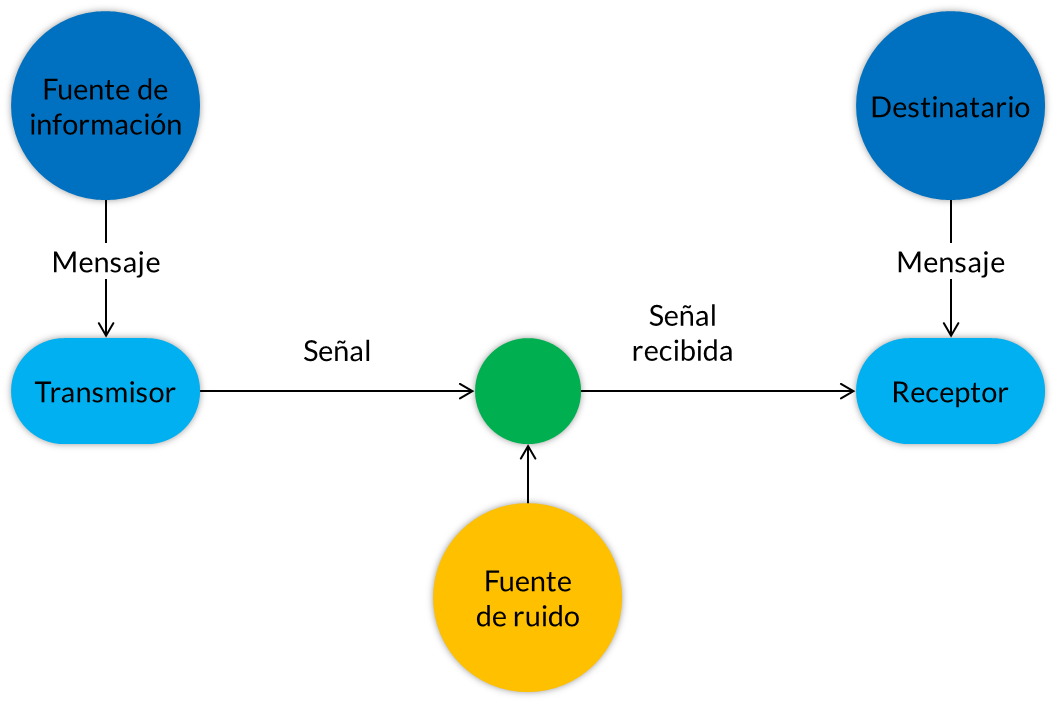
\includegraphics[width=0.6\columnwidth]{EsquemaShannon.png}
\caption{Diagrama de comunicación}
\end{center}
\end{figure}


A la hora de entablar una comunicación es necesario que las partes involucradas
se pongan de acuerdo sobre un lenguaje en común con el que van a desarrollar el
\quotes{dialogo} a lo largo del tiempo. Para poder llevar esto a cabo es que se
necesita definir un conjunto de símbolos $S = \{ s_1, ..., s_n \}$ que aporten
semantica a lo que se tratando de transmitir. De acuerdo al análisis de Shannon
cada uno de estos símbolos tiene asociada una cantidad de información que
responde a la formula $I(s_i) = log(\frac{1}{p(s_i)})$, donde $I(s_i)$ es la
información asociada a $s_i$ para cada $i$ con $1 \leq i \leq n$. Algo
importante a notar para entender esta formula es que la información de un
símbolo estará íntimamente relacionada con su probabilidad, a modo
coloquial, podemos pensar que en cuanto mas probable sea un símbolo, mas
esperable será su aparición, y por lo tanto mas predecible. En constraste
aquellas apariciones de símbolos poco probables son considerados un evento
desentonante con respecto a mucho mas usuales, por lo que se les da mas valor
semántico. En base a ello podemos observar que dicha definición cumple con
ciertas condiciones naturales para el calculo de de la información:

\begin{itemize}
	\item Si $p(s_i) = 1$ para algun $i$, entonces $I(s_i) = 0$, ya que un evento que ocurre siempre no aporta información significativa
	\item Si $s \in S$, entonces $I(s) \geq 0$. Esto vale ya que la inversa de la probabilidad es siempre mayor o igual a 1
\end{itemize}

\subsection{Entropía}

Ademas nos interesará otra noción importante, la de \textit{Entropía}. 
Esta refleja el promedio de la información
obtenida de una fuente en base a las probabilidad de ocurrencia e información
que provee cada símbolo en la comunicación, o, de otra manera, el nivel de
desorden de la comunicación.  

\begin{definicion} \label{eq:entropia}
Sea $S$ una fuente de información. Se define $H(S)$ la entropía de la fuente como a continuación.

\begin{equation} 
	H(S) = \sum\limits_{i=1}^n p(s_i)I(s_i)
\end{equation}

\end{definicion}

Por ejemplo, al ser todos los símbolos, igualmente probables,
la entropía será máxima alcanzando el valor de $log_2(\lvert simbolos\rvert)$.
De esta ultima observación se desprende, de forma general, que cuanto mayor sea el grado de
\quotes{equiprobabilidad} de los símbolos de la fuente, mayor será la
\textit{Entropía}, no superando al máximo posible (en el caso equiprobable).
Por el contrario sera mucho menor para aquellas fuentes en las
que la distribución de probabilidades sea muy desigual (siempre por encima de cero).
Esto será de vital importancia para los análisis posteriores.
\\

La longitud promedio de un código es $L(C) = \sum_{s \in S} P(s)l(C(s))$ donde
$l(C(s))$ es la largo de la codificación de S.
\\

\subsection{Compresibilidad}

Otra noción que se introduce en este trabajo es la de \textit{Compresibilidad}
\begin{definicion}
Sea $S$ una fuente de información, definimos el nivel de \textit{Compresibilidad} de S como
\begin{equation} \label{eq:eta_c}
	\eta_{C}(S)=\frac{H_{max}(S) - H(S)}{H_{max}(S)}
	\end{equation}donde $H(S)$ es la entropía de la
	fuente (ver Definición \ref{eq:entropia}) y $H_{max}(S)$ la entropía máxima.
\end{definicion}

Cuando $H(S) = H_{max}(S)$ decimos que
la fuente no es muy compresible debido a que la única forma optima e instantánea
de codificar los símbolos es que todos tengan la misma longitud. Por otro lado
si $H(S) << H_{max}(S)$ \footnote{Entiéndase $A << B$ como $A$ mucho menor que $B$} y asignamos a símbolos más frecuentes
una longitud mas chica que al resto. Permitiendo esto que la longitud promedio
sea menor y por tanto, la longitud promedio de los códigos que se transmitan
mucho mas bajos.
Es por eso que esta formula intenta representar el grado de compresión de la fuente.
Cuanto mas cercano este coeficiente es a cero o uno sera posible comprimir menos
o mas la fuente respectivamente.

\subsection{Protocolo ARP}
Durante los experimentos se analizaron los paquetes ARP. Estos tipo de paquetes
son de control interno de la red que permiten comunicar, mediante distintos mensajes,
que dirección \textbf{IP} le corresponde a qué dirección \textbf{MAC}. Cada dispositivo
cuenta con una caché de estas traducciones para poder efectivamente
transmitir paquetes \textbf{IP} (Capa 3, en el modelo \textbf{OSI}) por la red embebidos
en paquetes \textbf{MAC} (Capa 2, en el modelo \textbf{OSI}). Para esto existen
dos tipos de operaciones, \textit{who-has} e \textit{is-at}. Cuando un nodo A
de la red desea conocer cual es dispositivo B que tiene cierta \textbf{IP} (ie. 192.168.0.1)
éste transmite un mensaje \textit{broadcast} \textit{who-has} con el campo \emph{Target Protocol Address}:192.168.0.1.
Al dispositivo B, con esta IP, le llega este mensaje (eventualmente le llega a todos pero solo B responde ya que es el único con esta IP)
responde con el tipo de operación \textit{is-at} unicast a A (puede debido a que en el paquete está la dirección de source
que es la \textbf{MAC} address del dispositivo A). A A, le llega esta respuesta y con eso agrega a las traducciones esta IP con la respectiva mac adress
recibida. Las entradas de la caché cuentan con un tiempo de expiración debido a posibles cambios de IP de los dispositivos. Finalmente
es por esto último que pasado el tiempo de expiración se vuelve a realizar este protocolo \footnote{Este protocolo se describe en el RFC 826, ver en \url{https://tools.ietf.org/html/rfc826}}

\subsection{Paquetes de red}

En las redes de comunicación informáticas, la información se mueve a través de
ellas en forma de paquetes. Dichos paquetes cuentan con varios campos (se
agregan a medida que los paquetes viajan por el stack \textbf{OSI}, ver \cite[Capítulo 1, p.~32]{compnetworks}), en este
trabajo para modelar las fuentes nos interesaremos en los paquetes de tipo $Ethernet$ \footnote{O en su defecto 802.11 (en las redes Wi-Fi)} e $IP$. En el caso
de $Ethernet$, los campos son:

\begin{enumerate}
	\item MAC orgen
	\item MAC destino
\end{enumerate}

Mientras que en los paquetes ARP de capa 3 nos interesan los campos:

\begin{enumerate}
	\item MAC de origen
	\item IP de origen
	\item MAC de destino
	\item IP de destino
\end{enumerate}


\section{Metodologia}
\subsubsection{Protocolo \textbf{ICMP}}

\textbf{ICMP}\cite{rfc792} (\emph{Internet Control Message Protocol}) es un protocolo que
forma parte de la arquitectura \textbf{TCP/IP} pensado para mensajes de control
de Internet. Se utiliza en situaciones, y distintos propósitos como

\begin{itemize}
	\item Cuando un datagrama no puede alcanzar su destino
	\item Cuando un router no tiene la capacidad de forwardear este paquete
	\item Redirigir el host hacia una ruta más corta para el envio del paquete
	\item Se quiere comprobar que una maquína esta viva (\textbf{ping})
	\item Se quiere saber la ruta a un determinado host (\textbf{traceroute})
\end{itemize}

\begin{figure}[ht]
	\begin{center}
		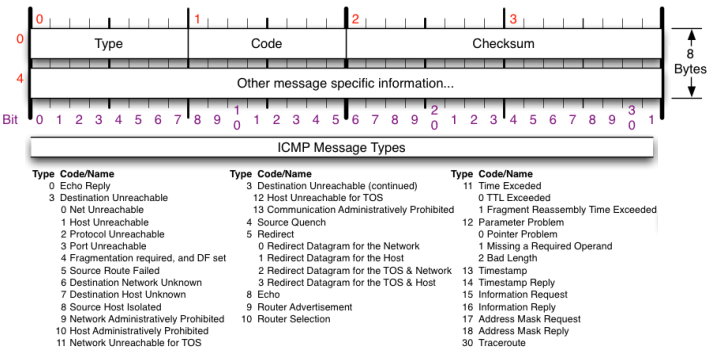
\includegraphics[width=0.8\columnwidth]{imagenes/icmp.png}
		\caption{Paquete ICMP}
		\label{fig:picmp}
	\end{center}
\end{figure}

En la figura \ref{fig:picmp} se ilustran los diferentes campos, junto con
las combinaciones de tipo/código de un paquete
ICMP. Para el desarrollo de este trabajo nos interesarán principalmente
el campo type, y más específicamente, dos valores que puede tomar durante
la determinación de la ruta que son, Echo Reply y
Time Exceeded. El paquete con tipo Time Exceeded lo envía el gateway al host
de salida cuando el campo TTL (\emph{Time to Live}) llega a cero y
por tanto debe descartar el forwadeo del datagrama original.


\subsection{Algoritmo Traceroute}

\subsubsection{Descripción del algoritmo}

\begin{figure}[ht]
	\begin{center}
		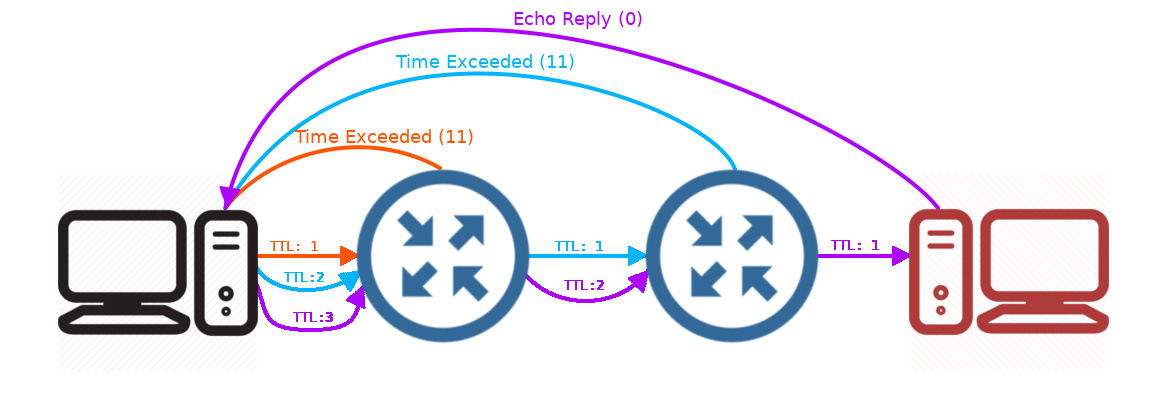
\includegraphics[width=0.6\columnwidth]{imagenes/diagrama_1.jpg}
		\caption{Diagrama de envió de paquetes del algoritmo}
		\label{fig:diagramasimple}
	\end{center}
\end{figure}

Sea $S$ el host que desea enviar el paquete y $T$ el host destino.
El algoritmo consiste en enviar desde $S$ al host de destino $T$ paquetes
\emph{Echo Request} con el campo $TTL=i$ en el datagrama \textbf{IP} para $i=1 \dots
MAX\_HOPS$ o hasta que se haya alcanzado al host $T$. Cada vez que el paquete
es forwardeado por un gateway al próximo gateway/host (Next Hope), este decrementará el
valor de este TTL. Cuando el valor llegue a cero el último gateway, llamémoslo
$M$, le informará mediante un paquete \textbf{ICMP} que el paquete fue expirado.
Como se ilustra en la figura \ref{fig:diagramasimple}, el gateway le responde con un paquete con el campo $tipo$ en
Time Exceeded (11) a $S$, obteniendo a su vez $S$ con esto, la \textbf{IP} de $M$ como
también la estimación del \textit{Round
Trip Time} (RTT) a este gateway $M$, y como se explicará luego el $RTT$ del enlace
del anterior gateway hasta este. Como esto se realiza reiteradas veces, en
cada paso, aumentando el TTL se llegan a conocer, en teoría, todos los
gateways, desde $S$, intermedios hasta llegar al destino $T$.

\subsubsection{Posibles problemas en la vida real}


Esto brinda en teoría una ruta efectiva bajo los supuestos de que
las rutas intermedias de forwarding se mantienen invariantes en el tiempo. En
la practica, esto no es usual dando a lugar a los siguientes inconvenientes

\begin{itemize}
	\item En cada salto es posible que cambien los gateways anteriores y siendo
	ademas imposible de detectar. Esto se puede ver en la figura \ref{fig:diagramareal},
	en donde el algoritmo, según el método, termina devolviendo una ruta incorrecta.
	\item El \textbf{RTT} estimado incluye al tiempo de encolamiento (es por esto
	que se le llama estimado) provocando una desviación significativa en las
	mediciones.
\end{itemize}

\begin{figure}[ht]
	\begin{center}
		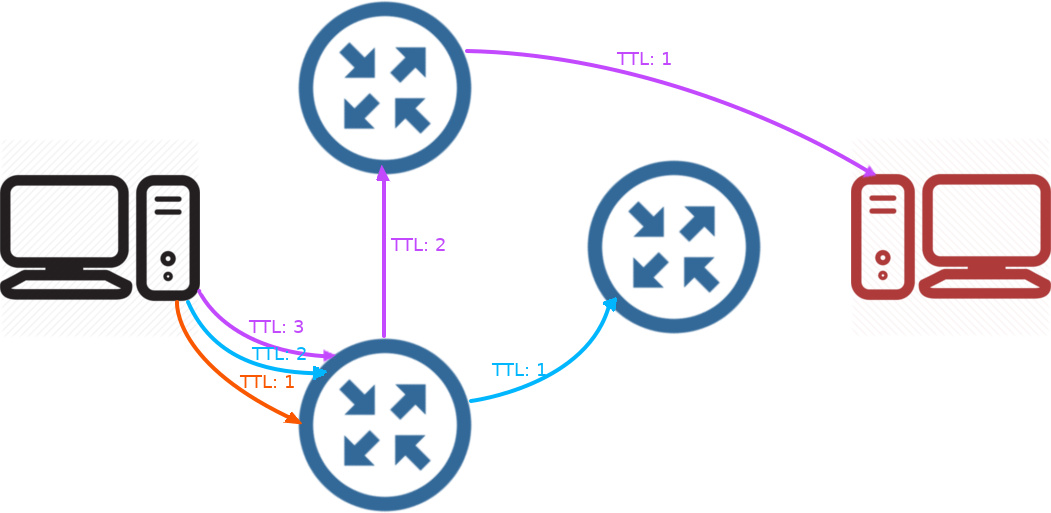
\includegraphics[width=0.6\columnwidth]{imagenes/diagrama_2.jpg}
		\caption{Diagrama de envió de paquetes del algoritmo}
		\label{fig:diagramareal}
	\end{center}
\end{figure}

Para solventar este tipo de problemas, para cada $TTL$ se envían varios paquetes
para luego obtener un valor promedio de $RTT$ mas significativo que el de un
solo intento, como a su vez, devolver solo la \textbf{IP} que respondió con mas
frecuencia.

Para calcular el $RTT$ del enlace promedio, se realiza la resta
del promedio del $RTT$ total obtenido en esta etapa con el promedio del $RTT$ total
de la etapa anterior.
Es decir

\begin{equation}
	\Delta RTT_{i} = \left\{
		\begin{array}{cl}
			\overline{RTT_{0}} & \mbox{si } i = 0\\
			\overline{RTT_{i}} - \overline{RTT_{i-1}} & \mbox{si } i > 0
		\end{array}
		\right.
\end{equation}

Cuando los tiempos de encolamiento y las rutas son invariantes en el tiempo
esta magnitud física siempre es positiva. Pero como, se mencionó anteriormente, esto
no siempre es así. La medida que toma el algoritmo en los casos cuando
$\Delta RTT_{i} < 0$ es la de descartar el
gateway y considerarlo como que forma parte del enlace.

\clearpage

\subsection{Determinación de enlace intercontinental}

\begin{figure}[ht]
	\begin{center}
		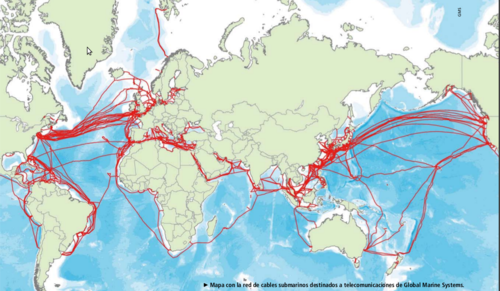
\includegraphics[width=0.6\columnwidth]{imagenes/mapa-transcontinental.png}
		\caption{Mapa con los cables intercontinentales existentes}
		\label{fig:cables_intercontinentales}
	\end{center}
\end{figure}

El objetivo de este algoritmo además de brindar la ruta, es el de detectar de
forma automática, cuando un enlace intermedio por el que es forwardeado el
paquete es uno que cruza dos continentes, debiéndose esto posiblemente a
que el cable físicamente es transatlántico (cables submarinos que cruzan el
atlántico, como se observa en la figura \ref{fig:cables_intercontinentales}). Por esto, agregamos el mapa conseguido en Internet sobre los cables
íntercontinentales existentes para poder utilizar a la hora de comparar con
los enlaces encontrados.

Una vez calculado el $\Delta RTT_{i}$ de cada enlace hasta llegar
al ultimo host se realiza la normalización (se los lleva a la distribución normal)
el valor de cada uno con la siguiente formula.

\begin{equation}\label{eq:z}
	Z_{i} = \lvert\frac{\Delta RTT_{i} - \overline{\Delta RTT}}{\sigma \left(\Delta RTT \right)}\rvert
\end{equation}

Este valor $Z_{i}$ es de vital importancia ya que nos dice, estadísticamente,
para $\Delta RTT_{i}$ cuantas desvaciones estándar se aleja de la media.
Combinando esto con el trabajo de John M. Cimbala\cite{cimbala} nos da una forma de
detectar cuando en un muestreo se presentó un outlier dependiendo también de la
cantidad de muestras. La aplicación que tiene en el trabajo realizado es que se
termina identificando cuando el $RTT$ del enlace es típicamente alto los que nos
proporciona un sofisticado criterio para detectar los enlaces
intercontinentales como se comprobará mas adelante en las siguientes secciones.


\section{Resultados}
En esta secci\'on, presentaremos los resultados obtenidos en los experimentos
utilizando lo definido en la secci\'on de desarrollo.

Se buscaron analizar en cada fuente tres tipos de redes segun su escala, es
decir redes pequeña, mediana y gran escala. Estas redes fueron
una hogareña, de unas oficinas, de un laboratorio de una Universidad.

En cada captura se almaceno todo los paquetes (con la placa de red
correspondiente en modo promiscuo) que se transmitieron por la red con el
sniffer desarollado como se menciono previamente. Luego analizados
automaticamente por el otro programa `analy\_data` para producir los graficos
que se presentan a continuación.

\subsection{Nodos distinguidos}

En cada experimento se analizaron las dos fuentes de información y se definió
un criterio para distinguir un nodo de cada red. Este criterio consta en que
será distinguido el símbolo con mas probabilidad de ocurrir o equivalentemente
el símbolo que tenga menor información.

\subsection{Hipotesis planteadas} \label{sec:hipotesis}

Las hipotesis o preguntas que se presentan en este trabajo son las siguientes:

Para la fuente $S_2$ es que estos nodos \quotes{distinguidos} son
nodos especiales como routers, access points, etc. dado que estos participan
en la mayor parte de las comunicaciones con la red como con el exterior.
Por lo cual esto nos daría un método (no 100\% confiable debido a casos
atípicos) de determinar los router en una red.

La segunda es que una red \textit{cableada} será
mas \quotes{compresible} que una \textit{wireless}. Para esto se mostró el
cociente de la $\frac{H_{MAX}(S)-H(S)}{H_{MAX}(S)}$ como se desarrollo en la Definicion \ref{eq:eta_c}
y se los comparo entre el mismo tipo de fuente de los distintos experimentos.

\subsection{Descripción de los Gráficos}

En cada experimentación se generaron tres tipos de resultados/gráficos.

\begin{itemize}
	\item Un gráfico que muestra una representación tipo torta de la fuente,
	esto es, la probabilidad de ocurrencia de cada símbolo.  \item Un gráfico
	tipo histograma que muestra para cada símbolo la información de este. Este
	gráfico cuenta además con una barra horizontal que muestra donde se sitúa
	la Entropía de la fuente (en color naranja) y otra barra similar que
	muestra donde se sitúa la Entropía máxima que podría tener la fuente.
	\item Un gráfico con la topología de los mensajes de la red. Donde los
	nodos son \textbf{MAC} address y las aristas representan un paquete de un
	nodo a otro
\end{itemize}

\clearpage
\subsection{Red hogareña}

En este caso se analizó una red de pequeña escala con 2 notebooks encendidas,
2 celulares y un router.


\subsubsection{Fuente Unicast-Multicast}

 Lo siguiente corresponde a la experimentación realizada para la fuente
 Unicast-Multicast en una red WiFi domestica.
 
\begin{figure}[hp!]
	\begin{minipage}[b]{0.9\linewidth}
		\subfloat[Probabilidades de los simbolos de la fuente $S_1$ para la red de hogareña]{
		 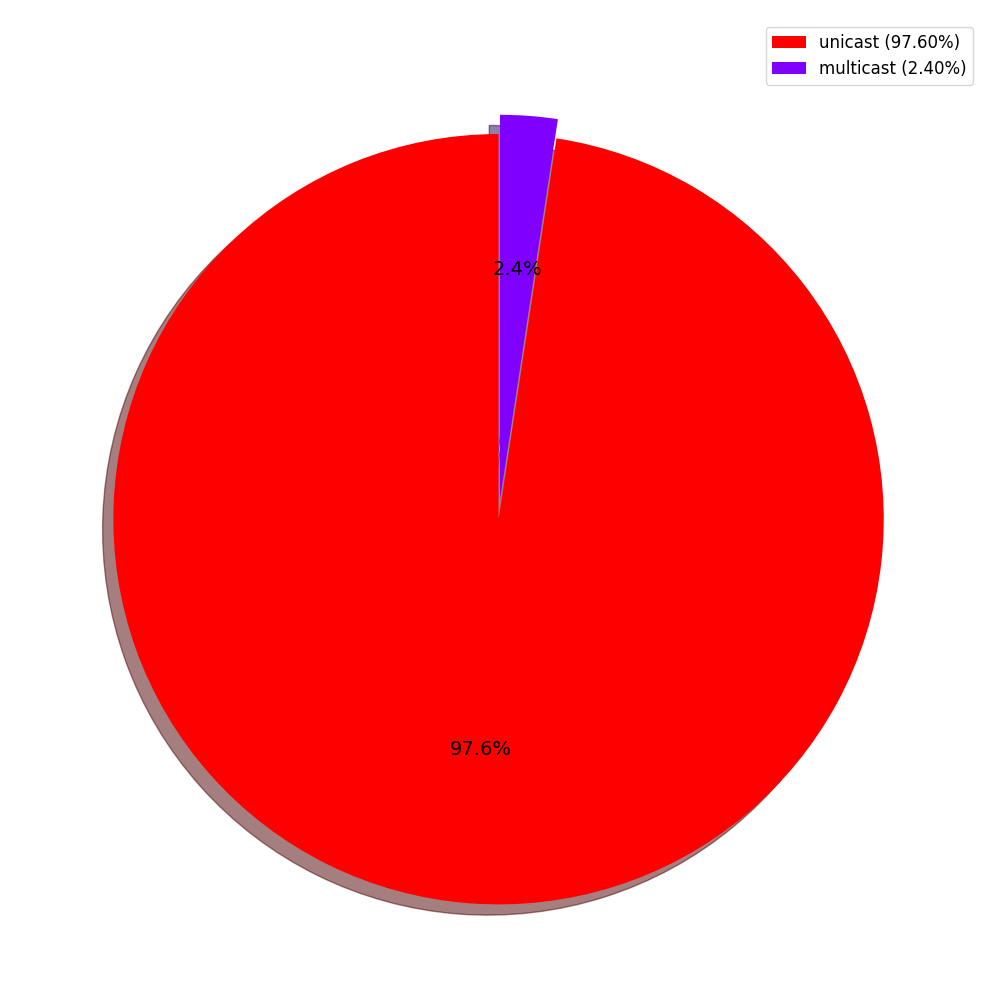
\includegraphics[width=0.45\linewidth]{../plots/mauro_s1_probabilidades.png}
		}
		\subfloat[Información de los simbolos de la fuente $S_1$ para la red de hogareña]{
		 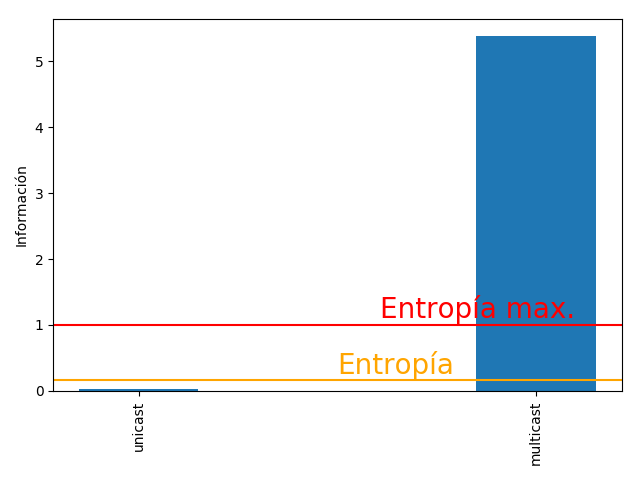
\includegraphics[width=0.55\linewidth]{../plots/mauro_s1_informacion.png}
		}
	\end{minipage}
\end{figure}


Como podemos ver los resultados obtenidos muestran una alta concentración de
paquetes \textit{multicast} por sobre los \textit{unicast}. En consecuencia la
entropía cae abruptamente, ya que como explicamos ésta se maximiza cuando la
distribución de las probabilidades de cada símbolo es equitativa, y baja a
medida que nos alejamos de ello. Nuestra primera impresión era que los
paquetes \textit{unicast} iban a predominar en la captura, sin embargo esto no
sucedió. Es posible que esto se deba a que la placa de red del dispositivo en
el cual se tomó la muestra no hayan entrado en modo promiscuo, en consecuencia
el \textit{sniffer} solo llego a capturar los paquetes cuyo destino era dicho
dispositivo (y no todos los \textit{unicast} transmitidos en la red). Por el
contrario los \textit{multicast} enviados por cualquier dispositivo de la red
se pudieron seguir escuchando sin ningún tipo de censura.

\subsubsection{Fuente ARP}

\begin{figure}[hp!]
	\begin{minipage}[b]{0.9\linewidth}
		\subfloat[Probabilidades de los simbolos de la fuente $S_2$ para la red de hogareña]{
		 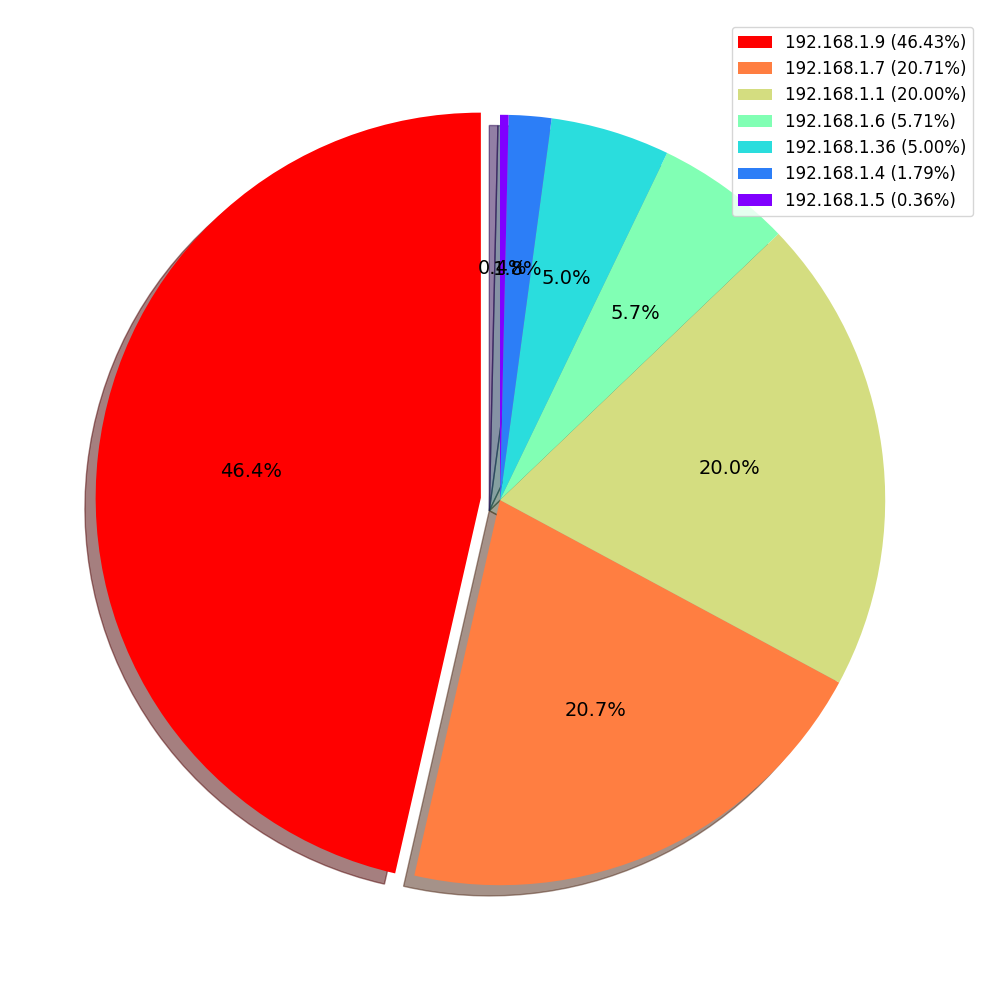
\includegraphics[width=0.45\linewidth]{../plots/mauro_s2_probabilidades.png}
		}
		\subfloat[Información de los simbolos de la fuente $S_2$ para la red de hogareña]{
		 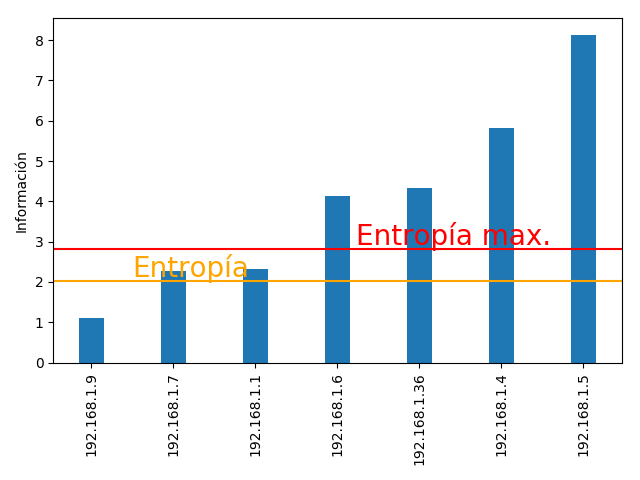
\includegraphics[width=0.55\linewidth]{../plots/mauro_s2_informacion.png}
		}
	\end{minipage}
\end{figure}

Este experimento lamentablemente no dio como esperábamos. La IP 192.168.1.9, se corresponde
a la notebook en la cual se corrió este experimento y no al router. La misma concentro aproximadamente
la mitad de los paquetes ARP de esta red y alcanza 1 de información.


\subsubsection{Topolog\'ia de la Red}
\begin{figure}[hp!]
	\begin{center}
	 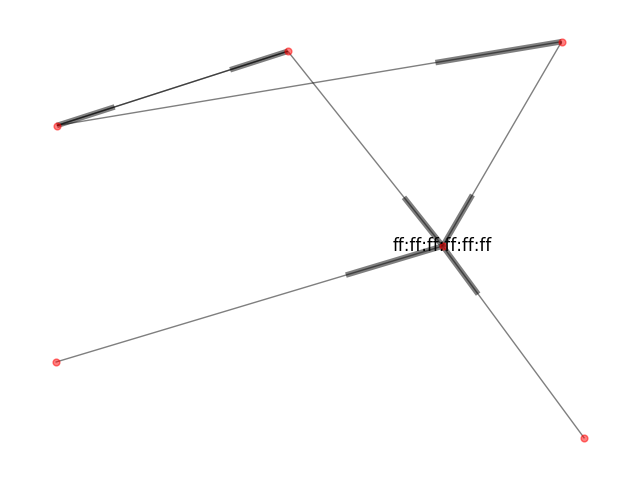
\includegraphics[scale=0.6]{../plots/mauro_s2_topologia.png}
	\end{center}
\end{figure}

Tiene una topolog\'ia estrella como es común en una red domestica. Del grafo se desprende que el nodo de mas a la izquierda y
arriba tiene la rareza de que nunca envió un \textit{who-has}, pero si respondió \emph{is-at} a dos nodos de la red.

\subsection{\emph{Red de Oficinas}}

En esta caso se analizo una red cableada de mediana escala, que consta de 6
oficinas con varias computadoras de escritorio (Desktop). Además en cada
oficina se encuentra un switch que conecta todas las PCs de esta. La captura
que se tomó fue de una hora para poder obtener estadísticamente suficiente
precisión en las medidas y que estas no sean alteradas por posibles `outliers`.

\subsubsection{Fuente Unicast-Multicast}

\begin{figure}[hp!]
	\begin{minipage}[b]{0.9\linewidth}
		\subfloat[Probabilidades de los simbolos de la fuente $S_1$ para la red de oficinas]{
		 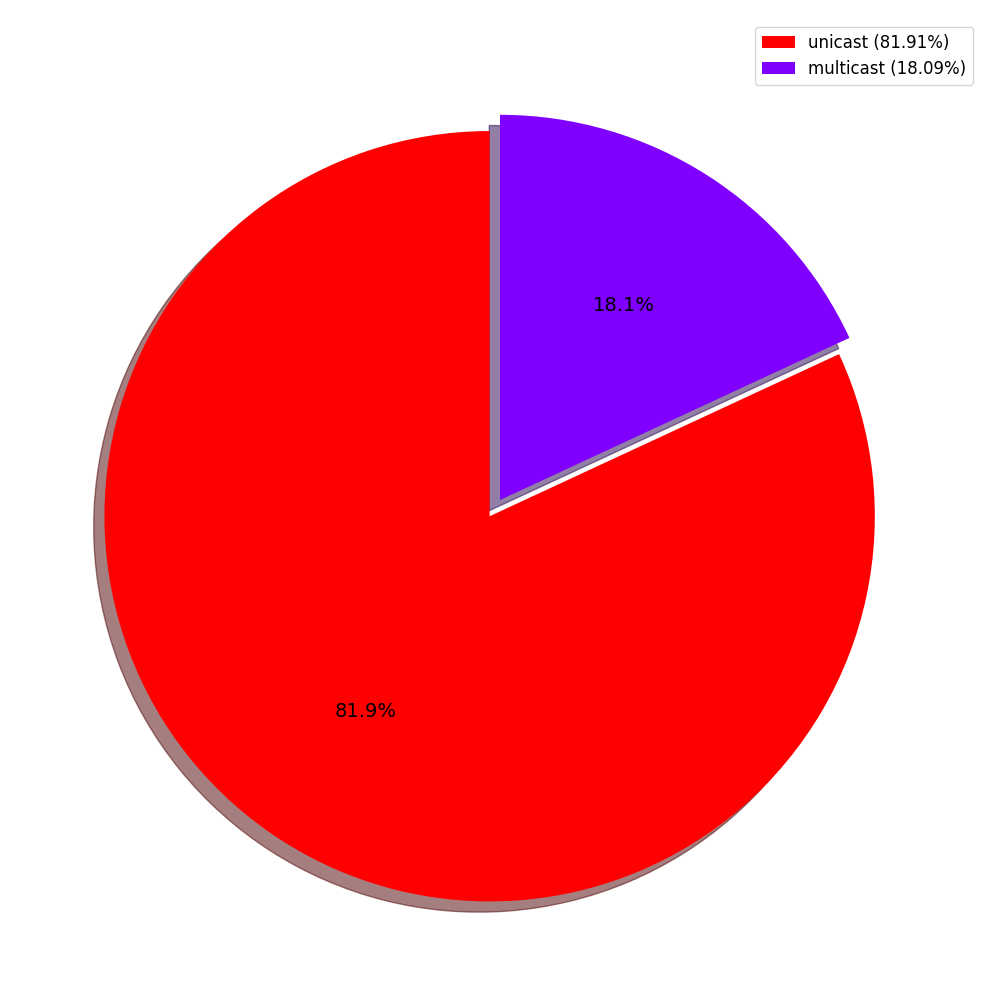
\includegraphics[width=0.45\linewidth]{../plots/trabajo_s1_probabilidades.png}
		}
		\subfloat[Información de los simbolos de la fuente $S_1$ para la red de oficinas]{
		 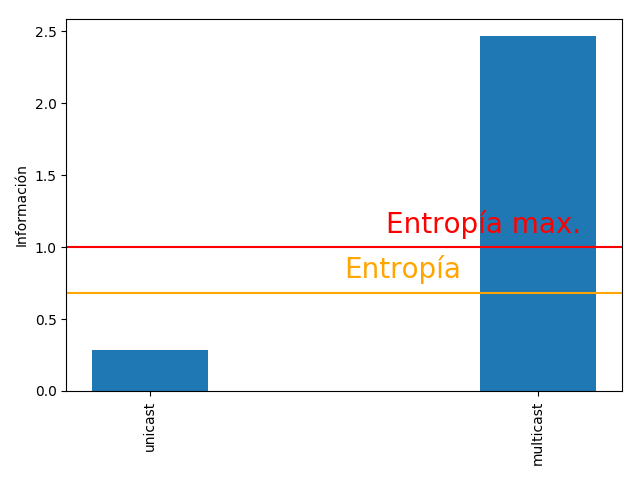
\includegraphics[width=0.55\linewidth]{../plots/trabajo_s1_informacion.png}
		}
	\end{minipage}
\end{figure}


Como se puede observar en ambos gráficos el el símbolo destacado es el
\textbf{unicast}, ya que este tiene mayor probabilidad y menor cantidad de
información. Esto nos dice que sobre el cable el $81.91\%$ los
paquetes fueron unicast.  El sentido de esto puede deberse a que los únicos
protocolos que usan el tipo de mensajes broadcast son protocolos de control y
representan una pequeña proporción del trafico total de la red.

\subsubsection{Fuente ARP}

\begin{figure}[hp!]
	\begin{minipage}[b]{0.9\linewidth}
		\subfloat[Probabilidades de los simbolos de la fuente $S_2$ para la red de oficinas]{
		 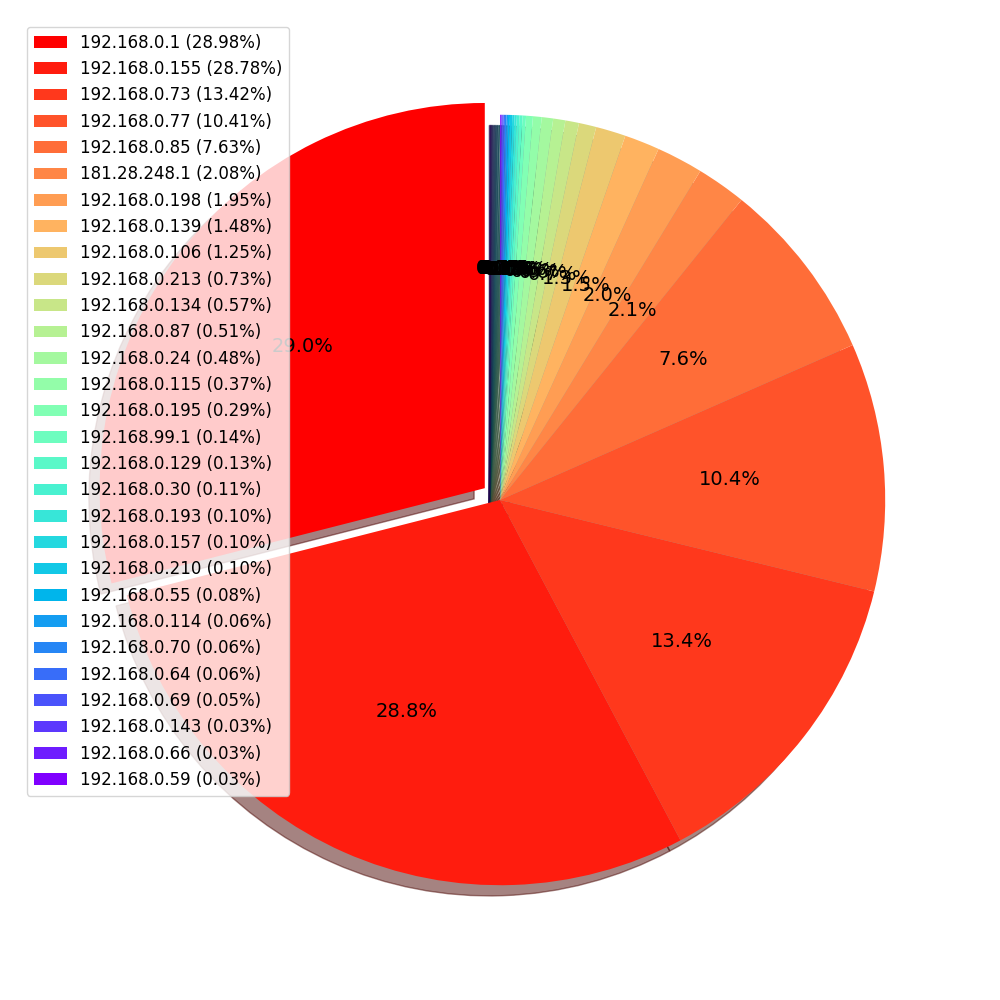
\includegraphics[width=0.45\linewidth]{../plots/trabajo_s2_probabilidades.png}
		}
		\subfloat[Información de los simbolos de la fuente $S_2$ para la red de oficinas]{
		 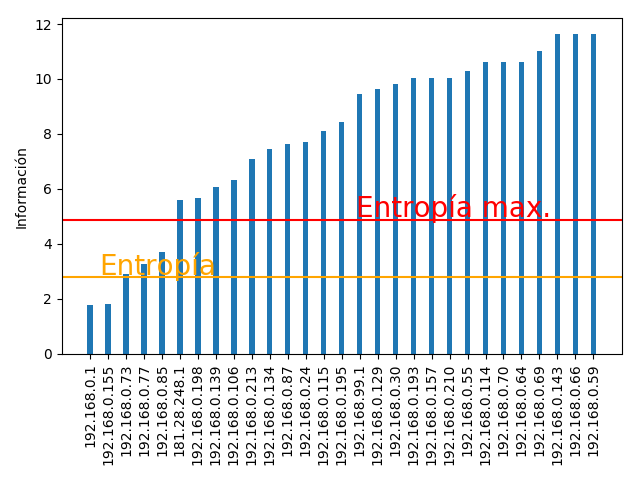
\includegraphics[width=0.55\linewidth]{../plots/trabajo_s2_informacion.png}
		}
	\end{minipage}
\end{figure}

En estos gráficos se puede ver que efectivamente el nodo \textbf{192.168.0.1}
es el destacado. Por previo conocimiento de la red se sabe que este
es el router lo cual refuerza nuestra hipótesis sobre los nodos destacados.
También se observa que la entropía alcanzada es de $2.77$ cuando la máxima
es $4.85$ y por tanto $\eta_{C} = 0.41$

\subsubsection{Topolog\'ia de la Red}
\begin{figure}[hp!]
	\begin{center}
	 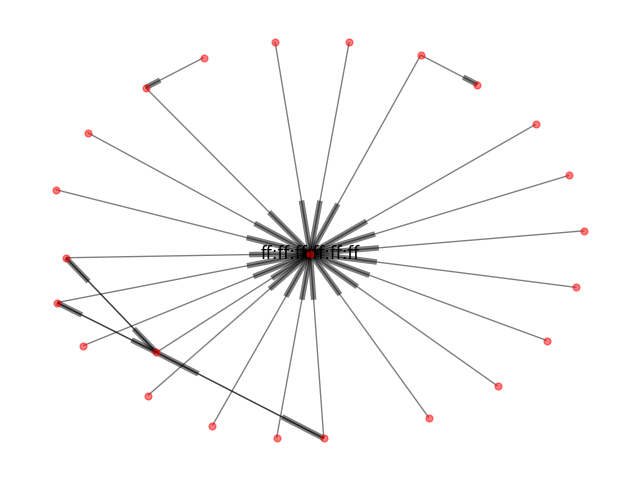
\includegraphics[scale=0.6]{../plots/trabajo_s2_topologia.png}
	\end{center}
\end{figure}

Se observa que la topología de mensajes arp es de tipo estrella
y que el grafo es conexo. El nodo del centro resulta ser la MAC ff:ff:ff:ff:ff:ff
es decir los mensajes broadcast. Se ve que hay pocos nodos que le hayan
enviado un paquete arp a otro que no sea el broadcast. Esto se debe
a que al estar detrás de un switch, los mensajes unicast de respuesta (\textit{is-at})
no son forwardeados a la interfaz de la maquina que realiza la captura aun
estando en modo promiscuo .En cambio cuando se trate de un mensaje unicast que
responde el mismo dispositivo que realiza la captura este si es registrado. Aun
asi se filtran mensajes unicast de pc's a otras pc's. Esto como se dijo puede
deberse a switchs que no aprendieron bien la tabla de forwardeo.

\subsection{Red de Laboratorios del DC}

Este experimento fue realizado en una red de gran escala a las 16:00 hs durante media hora en los Laboratorios del DC.

\subsubsection{Fuente Unicast-Multicast}

\begin{figure}[hp!]
	\begin{minipage}[b]{0.9\linewidth}
		\subfloat[Probabilidades de los simbolos de la fuente $S_1$ para la red de laboratorios]{
		 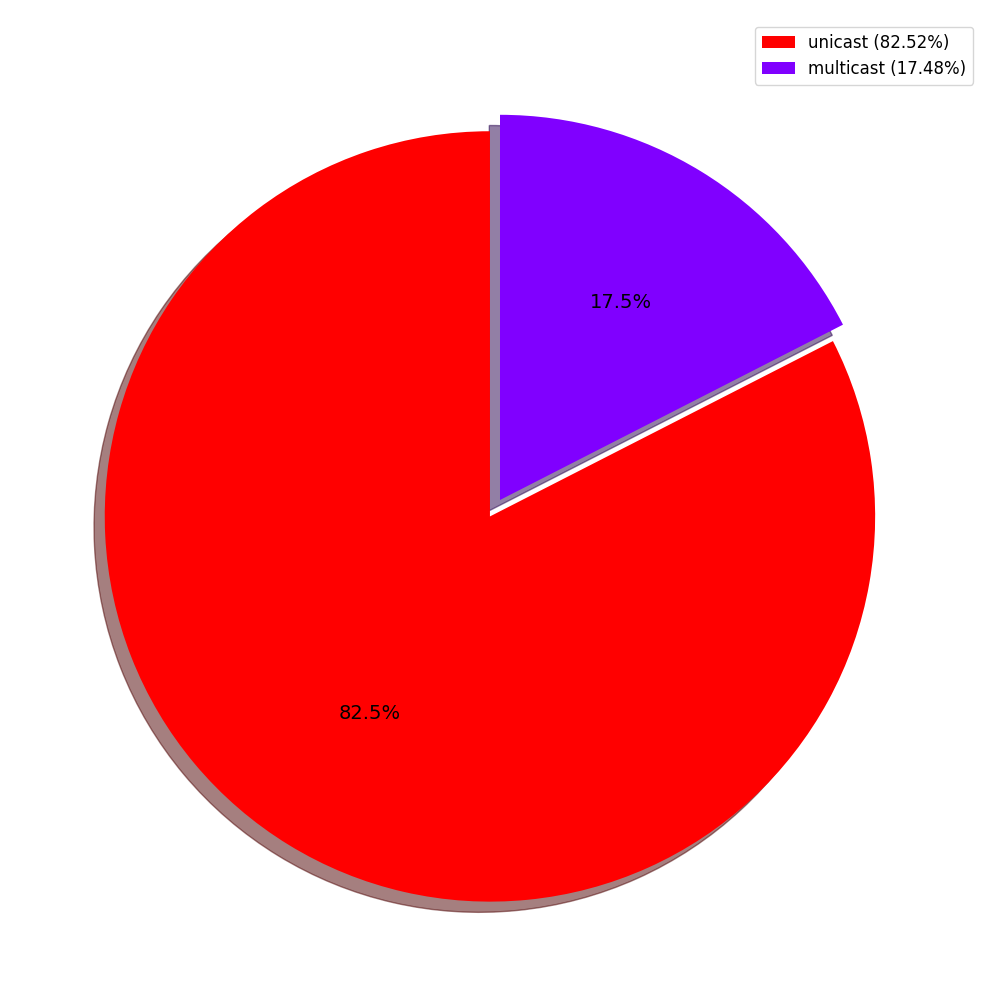
\includegraphics[width=0.45\linewidth]{../plots/labos_s1_probabilidades.png}
		}
		\subfloat[Información de los simbolos de la fuente $S_1$ para la red de laboratorios]{
		 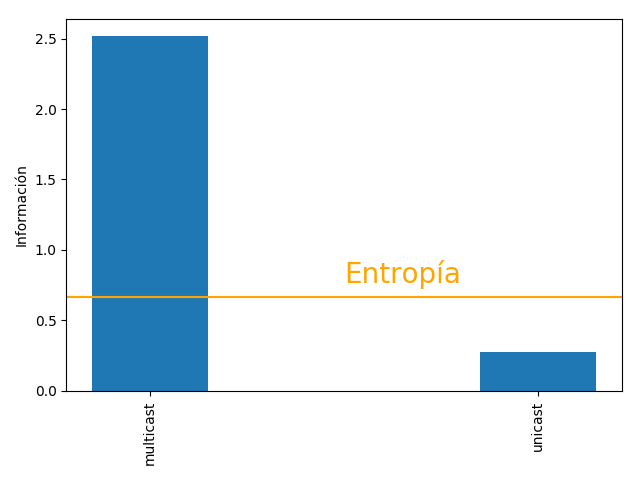
\includegraphics[width=0.55\linewidth]{../plots/labos_s1_informacion.png}
		}
	\end{minipage}
\end{figure}

Como se dijo anteriormente en el caso de la Red de Oficinas, se ve que la mayor\'ia
de los paquetes son unicast porque los paquetes broadcast son usados generalmente
por los protocolos de control. Ademas, la probabilidad de unicast fue de 0.82, la
informacion de 0.27 y la entropia de la fuente de 0.66.

\subsubsection{Fuente ARP}

\begin{figure}[hp!]
	\begin{minipage}[b]{0.9\linewidth}
		\subfloat[Probabilidades de los simbolos de la fuente $S_2$ para la red de laboratorios]{
		 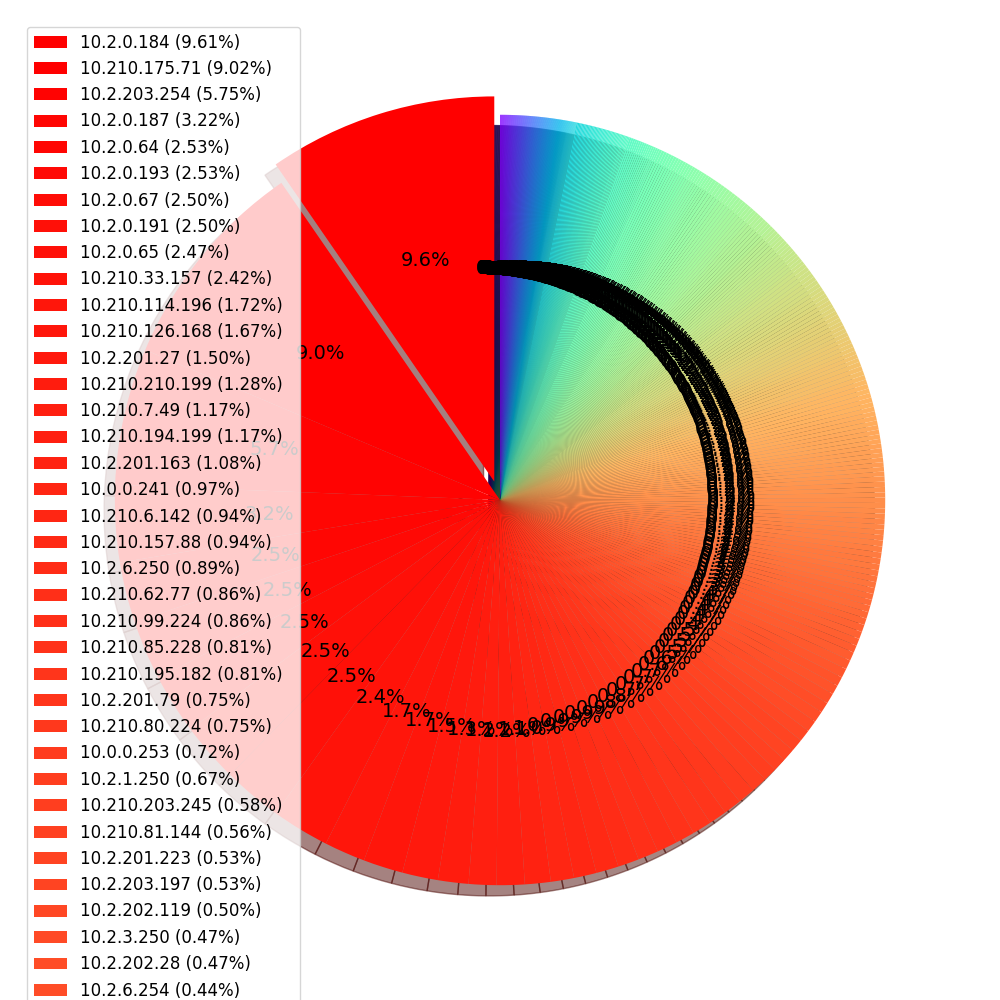
\includegraphics[width=0.45\linewidth]{../plots/labos_s2_probabilidades.png}
		}
		\subfloat[Información de los simbolos de la fuente $S_2$ para la red de laboratorios]{
		 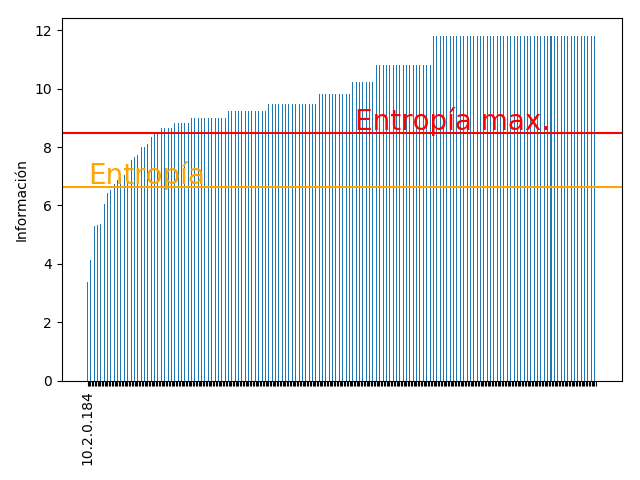
\includegraphics[width=0.55\linewidth]{../plots/labos_s2_informacion.png}
		}
	\end{minipage}
\end{figure}

Podemos observar que en este caso el nodo destacado es de la IP 10.2.0.184 con casi el 10\%.
Investigamos a que dispositivo corresponde y resulta ser la impresora, lo que nos hace pensar que
por el horario se estaba usando mucho para imprimir, aunque también podría ser
que su tabla ARP tiene una cache con poco tiempo de vida para cada elemento.

En cuanto a la entropía, vemos que es de 6.619, el máximo de 8.484 y la comprensibilidad es
de 0.220.

\subsubsection{Topolog\'ia de la Red}

\begin{figure}[hp!]
	\begin{center}
	 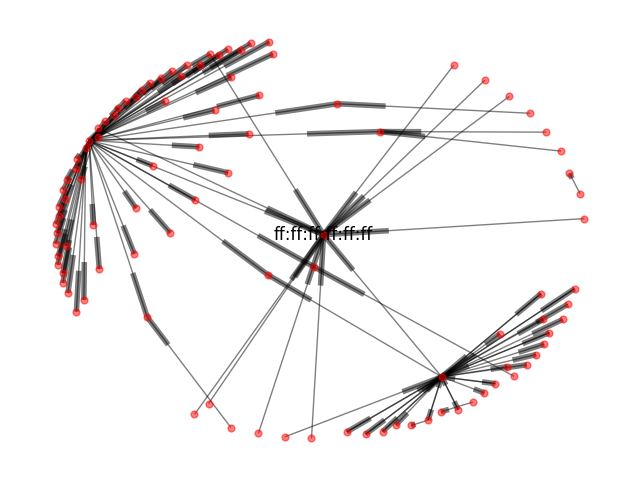
\includegraphics[scale=0.6]{../plots/labos_s2_topologia.png}
	\end{center}
\end{figure}

Como vemos, es nuevamente del tipo estrella la topología como es esperada. Notamos una densidad
distinta de nodos en varias regiones que se pueden observar. Creemos que esto se puede deber
a la disposición de cada laboratorio y los distintos routers o access-points que están ubicados en la zona.
Otra observación es que se pueden ver dos nodos arriba a la derecha de la red que no son conexos al resto del grafo.


\subsection{Comentarios generales}

\begin{figure}[hp!]
	\centering
	\begin{tabular}{|c|c|c|c|c|}
		\hline
		Red & Tipo & Entropía & Entropía Max & $\eta_{C}$ \\
		\hline
		Oficinas & Cableada & 2.777 & 4.858 & 0.428 \\
		\hline
		Hogareña & Wifi & 2.034 & 2.807 & 0.276 \\
		\hline
		Laboratorios & Wifi & 6.619 & 8.484 & 0.220 \\
		\hline
	\end{tabular}
	\caption{Entropía vs Max Entropía de las fuentes $S_2$ de las redes}
	\label{fig:tabla}
\end{figure}

En la figura \ref{fig:tabla} se pueden ver que las redes wifi son menos compresibles ($\eta_{C}=0.276$ y $\eta_{C}=0.220$)
con respecto a la cableado ($\eta_{C}=0.428$). Esto reafirma nuestra hipótesis (ver Sección \ref{sec:hipotesis}) de que las redes cabledas son más compresibles que
las redes wifi.


\section{Conlusiones}
A modo general pudimos observar que en el caso
de la primer fuente, en todas las redes el 
símbolo destacado, o mas probable, es el unicast.
Como ya se explicó previamente esto puede deberse
a la poca cantidad de paquetes de control que suceden
en la red con respecto a la totalidad de paquetes.


Se confirmaron las hipótesis que se presentaron sobre los nodos destacados de
la fuente $S_2$. Es decir, todos estos, tenían algún propósito especial para la
red (router, impresora, access points, etc.) como lo de los niveles
de compresibilidad de los distintos tipos de redes (Cableada, Wifi).


Otra punto importante es qué se observo en todas las redes una
menor cantidad de dispositivos en el gráfico de la topología
que IP's en los gráficos de probabilidad e información de la fuente $S_2$.
Esto puede deberse a que haya nodos que tenga varias IP's
o que se enviaron mensajes \textit{who-has} con IP's que no existían o dejaron
de existir en la red.

Para concluir, nos divirtió analizar las distintas redes y poder elaborar hipótesis
y comprobar resultados de los experimentos realizados. De esta forma pudimos iteriorizarnos
y comprender mejor las redes que utilizamos habitualmente.


\section{Bibliografía}
\begin{thebibliography}{9}

\bibitem{compnetworks}
  Larry L.Peterson and Bruce S. Davis,
  \emph{Computer Networks: A Systems Approach},
  Morgan Kaufmann,
  5th edition,
  2011.
\bibitem{shannon}
	Claude E. Shannon,
	\emph{A Mathematical Theory of Communication},
	The Bell System Technical Journal,
	1984,
	\url{http://math.harvard.edu/~ctm/home/text/others/shannon/entropy/entropy.pdf}
\end{thebibliography}



\end{document}
